\documentclass{article}
\usepackage{amsmath}
\usepackage[utf8]{inputenc}
\usepackage{pgfplots}
\usepackage{listings}
\usepackage[utf8]{inputenc}
\usepackage{graphicx}

\graphicspath{ {../results/} }

\lstset{
	basicstyle=\footnotesize,
	numbers=left,
	tabsize=3,
	title=\lstname,
	breaklines=true
}

\addtolength{\oddsidemargin}{-.875in}
\addtolength{\evensidemargin}{-.875in}
\addtolength{\textwidth}{1.75in}

\addtolength{\topmargin}{-.875in}
\addtolength{\textheight}{1.75in}

\title{Lernverfahren autonomer Roboter - Übung 7}
\author{Tobias Hahn\\ 3073375}	
	
\begin{document}
\maketitle
\newpage
\section*{Übung 7}
\section{Normal Equation}

\begin{equation}
	\begin{split}
	X & = 
		\begin{bmatrix}
			1 & 1 \\
			1 & 2 \\
			1 & 4 \\
			1 & 5 \\
			1 & 8 
		\end{bmatrix} \\
	y & = 
		\begin{bmatrix}
			3.5 \\
			2.5 \\
			5.5 \\
			9.5 \\
			14.5
		\end{bmatrix}
	\end{split}
\end{equation}

\begin{equation}
	X^t X = 
	\begin{bmatrix}
		1 & 1 & 1 & 1 & 1 \\
		1 & 2 & 4 & 5 & 8
	\end{bmatrix} * 
	\begin{bmatrix}
		1 & 1 \\
		1 & 2 \\
		1 & 4 \\
		1 & 5 \\
		1 & 8 
	\end{bmatrix} =
	\begin{bmatrix}
		5 & 20 \\
		20 & 110
	\end{bmatrix}
\end{equation}

\begin{equation}
	(X^t X)^{-1} = 
	\begin{bmatrix}
		5 & 20 \\
		20 & 110
	\end{bmatrix}^{-1} =  
	\frac{1}{550-400} *
	\begin{bmatrix}
		110 & -20 \\
		-20 & 5
	\end{bmatrix} = 
	\begin{bmatrix}
		\frac{11}{15} & -\frac{2}{15} \\
		-\frac{2}{15} & \frac{1}{30}
	\end{bmatrix}
\end{equation}

\begin{equation}
	(X^t X)^{-1} X^t = 
	\begin{bmatrix}
		\frac{11}{15} & -\frac{2}{15} \\
		-\frac{2}{15} & \frac{1}{30}
	\end{bmatrix} * 
	\begin{bmatrix}
		1 & 1 & 1 & 1 & 1 \\
		1 & 2 & 4 & 5 & 8
	\end{bmatrix} =
	\begin{bmatrix}
		\frac{3}{5} & \frac{7}{15} & \frac{1}{15} & \frac{1}{15} & -\frac{1}{3} \\
		\frac{1}{10} & -\frac{1}{15} & 0 & \frac{1}{30} & \frac{2}{15}
	\end{bmatrix}
\end{equation}

\begin{equation}
	\hat\omega = (X^t X)^{-1} X^t y = 
	\begin{bmatrix}
		\frac{3}{5} & \frac{7}{15} & \frac{1}{15} & \frac{1}{15} & -\frac{1}{3} \\
		\frac{1}{10} & -\frac{1}{15} & 0 & \frac{1}{30} & \frac{2}{15}
	\end{bmatrix} * 
	\begin{bmatrix}
		3.5 \\
		2.5 \\
		5.5 \\
		9.5 \\
		14.5
	\end{bmatrix} =
	\begin{bmatrix}
		-\frac{17}{30} \\
		\frac{73}{30}
	\end{bmatrix}
\end{equation}

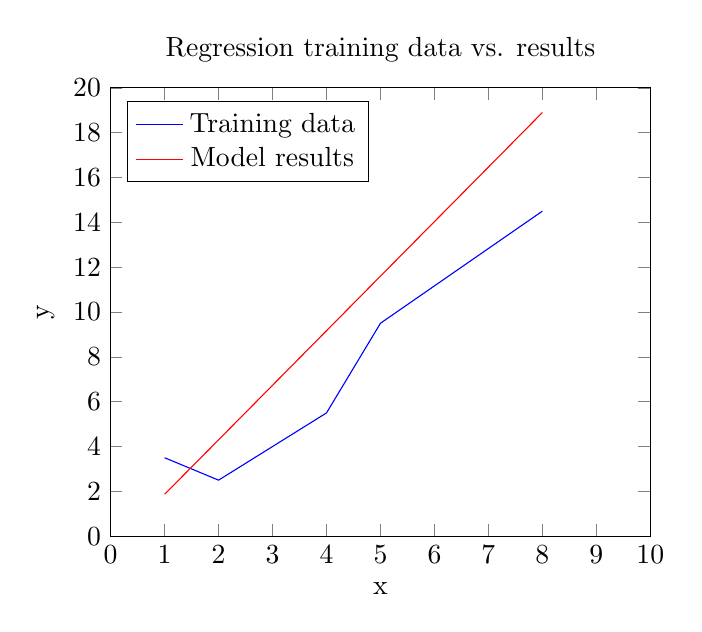
\begin{tikzpicture}
\begin{axis}[
    title={Regression training data vs. results},
    xlabel={x},
    ylabel={y},
    xmin=0, xmax=10,
    ymin=0, ymax=20,
    xtick={0,1,2,3,4,5,6,7,8,9,10},
    ytick={0,2,4,6,8,10,12,14,16,18,20},
	legend pos=north west,
]
 
\addplot[
    color=blue,
    mark=cross,
    ]
    coordinates {
    (1,3.5)(2,2.5)(4,5.5)(5,9.5)(8,14.5)
    };

\addplot[
    color=red,
    mark=cross,
    ]
    coordinates {
    (1,28/15)(2,43/10)(4,55/6)(5,58/5)(8,189/10)
    };
    \legend{Training data, Model results}
 
\end{axis}
\end{tikzpicture}

\section{Normal Equation}
Folgend der Code und die Ausgaben des Programms:

\subsection{Code}
\lstinputlisting{../code/regression.py}
\subsection{Results}
\begin{figure}[h]
    \centering
    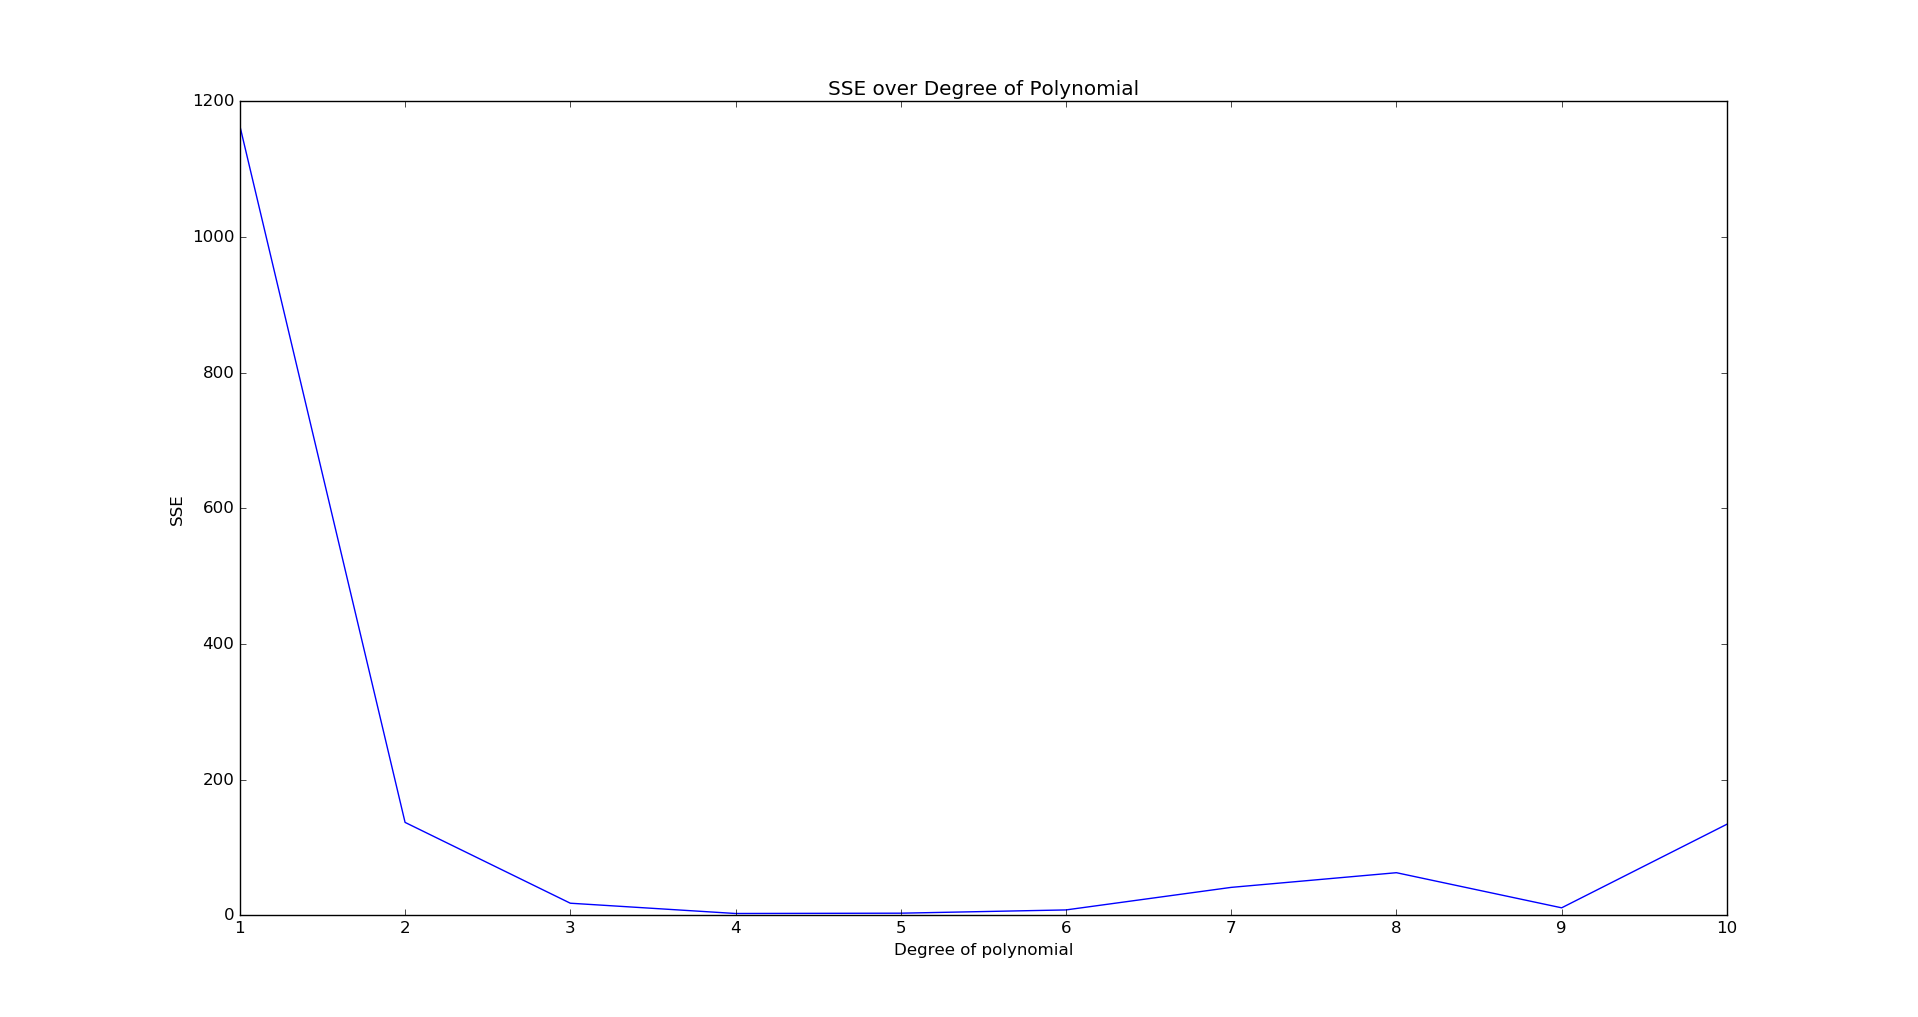
\includegraphics[width=\textwidth]{SSE.png}
\end{figure}
\begin{figure}[h]
    \centering
    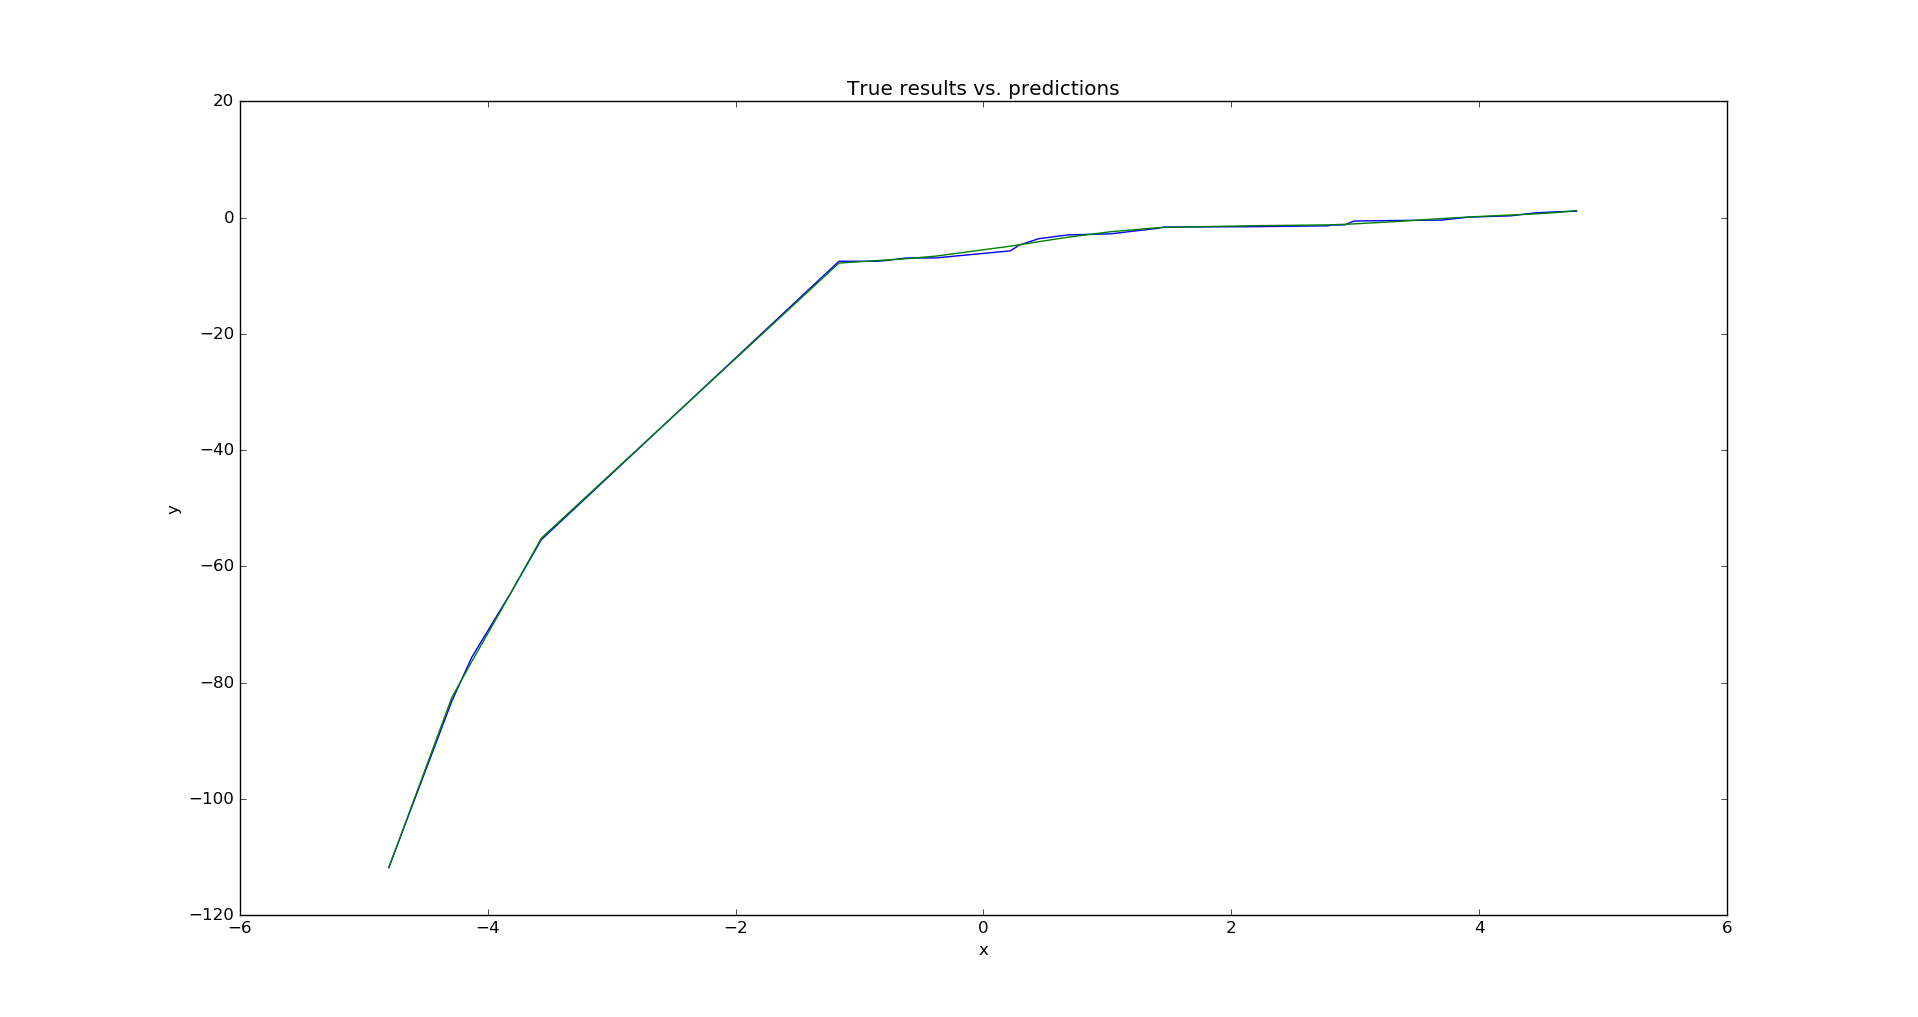
\includegraphics[width=\textwidth]{RESULTS.png}
\end{figure}
\end{document}
